\chapter{Analogical recommendation}
\label{CHAP:analogical_recommendation}
\localtableofcontents*
\vspace*{\baselineskip}

\initial{N}ow that we have enough background on recommender systems, we are in
a position to present our contribution to analogical recommendation.\\

This chapter is structured as follows. In Section
\ref{SEC:analogical_reco_basic_algo}, we will describe our first approach which is
directly inspired from extended classifiers, and compare it to the
neighborhood approach and matrix factorization-based techniques. In Section
\ref{SEC:clone_based_view} we will devise a new algorithmic framework that is still
inspired by analogy, but that does not rely on the search of $3$-tuples which
will appear to be very costly. Finally in Section
\ref{SEC:mining_analogical_proportions}, we will address the problem of mining
analogical proportions in partially described databases, and describe how the
solving of this problem can be applied to a recommendation task. This will also
help us to retrospectively analyze the results obtained in Section
\ref{SEC:analogical_reco_basic_algo}.

\section{An algorithm using arithmetic proportion}
\label{SEC:analogical_reco_basic_algo}
We will here describe our first attempt to use an analogical proportion-based
algorithm for recommender systems. Let us note that applying analogical
reasoning to the task of recommendation has already been addressed in
\cite{SakAkaOkaDatTakKamMiyTsu11}, though with a significantly different
concern. The main idea of our algorithm is quite
simple and is directly inspired by the analogical classifiers that we have
extensively studied in Chapter \ref{CHAP:functional_definition}.

\subsection{Algorithm}

Here again, we will make use of the analogical inference principle, but we will
state it in slightly different terms. In chapters
\ref{CHAP:formal_analogical_proportions} and \ref{CHAP:functional_definition},
the analogical inference principle stated that if four vectors $\mathbf{a},
\mathbf{b}, \mathbf{c}, \mathbf{d}$ are in proportion, then their labels should
also be in proportion.  Here, we will say that if an analogical proportion
stands between four users $a, b, c, d$, meaning that for each item $j$ that
they have commonly rated, the analogical proportion $r_{aj} : r_{bj} :: r_{cj}
: r_{dj}$ holds, then it should also hold for an item $i$ that $a, b, c$ have
rated but $d$ has not (i.e. $r_{di}$ is the missing component):
$$
\inferrule{r_{aj} : r_{bj} :: r_{cj} : r_{dj} ~~ \forall j \in
I_a \cap I_b \cap I_c \cap  I_d}
{r_{ai} : r_{bi} :: r_{ci} : r_{di} ~~ \forall i \in I_a \cap I_b \cap I_c,
\text{ and } i\notin I_d }
$$
This leads us to estimate $r_{di}$ as the solution $y$ of the following
analogical equation:
$$r_{ai} : r_{bi} :: r_{ci} : y.$$
Naturally, we may find many $3$-tuples $(a, b, c)$ that are in proportion with
$u$, so we will need  to aggregate all the candidate solutions $y$.  Given a
pair $(u,i)$ such that $\rui \notin R$, the main procedure to estimate $\rui$
is as follows:
\begin{enumerate}
\item Find the set of 3-tuples of users $a, b, c$ such that an analogical
  proportion stands between $a, b, c,$ and $u$ and such that the equation
    $r_{ai} : r_{bi} :: r_{ci} : y$ is solvable.
\item Solve the equation $r_{ai} : r_{bi} :: r_{ci} : y$ and consider the
  solution $y$ as a candidate rating for $r_{ui}$.
\item Set $\hat{r}_{ui}$ as an aggregate of all candidate ratings.
\end{enumerate}

This pseudo-algorithm is exactly that of a conservative classifier described in
Section \ref{SEC:conservative_classifier}, except that here, the instance space
(i.e. the space of $a, b, c, u$) changes with every pair $(u, i)$, and every
$3$-tuple $(a, b, c)$.

In our implementation, we have used the arithmetic proportion in
$\mathbb{R}^m$: $a:b::c:u \iff a - b = c - u$.  The four users $a, b, c, u$ are
here considered as vectors of ratings in a space defined by their common items.
For the sake of clarity though, we will not write them with boldface letters
and $a$ will denote both the user $a$ as well as its vectorial representation.
Let us consider Figure \ref{FIG:analogical_recommendation}: the four users $a,
b, c$ and $u$ are in proportion, i.e. they make up a parallelogram in the
2-dimensional space of their common items, namely the two movies Titanic and Toy story. If the
three users $a, b, c$ have rated a movie $i$ that $u$ has not rated, the
estimation of $\rui$ will be such that $a, b, c$ and $u$ still make up a
parallelogram, but this time in a 3-dimensional space. This process is also
explained in Table \ref{TAB:analogical_recommendation}.

\begin{figure}[!h]
\centering
  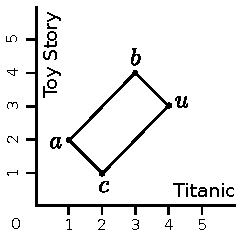
\includegraphics[width=2.5in]{figures/analogical_recommendation.pdf}
  \caption{Four users $a, b, c, u$ that are in proportion.}
\label{FIG:analogical_recommendation}
\end{figure}

\begin{table}[h!]
\centering
  \begin{tabular}{ c   c  c  c  c  c  }
\toprule
 & $j_1$ & $j_2$ & $j_3$ & $\cdots$ & $i$\\
  \midrule
$a$ & 1 & 4  & 3 & $\cdots$ & 2 \\
$b$ & 5 & 2  & 3 & $\cdots$ & 4 \\
$c$ & 1 & 5  & 3 & $\cdots$ & 3 \\
$u$ & 5 & 3  & 3 & $\cdots$ & ? \\
\bottomrule
\end{tabular}
\caption{The four users $a, b, c, u$ are in proportion for every item $j$ that
  they have commonly rated. For an item $i$ that $u$ has not rated, the
  prediction $\predrui$ is set as the solution of the analogical equation
  $2:4::3:?$, i.e. $\predrui = 3 - 2 + 4 = 5$, using the arithmetic proportion.}
\label{TAB:analogical_recommendation}
\end{table}

Just like with the conservative classifier, we will face the problem that in
practice, we may not find any $3$-tuple $(a, b, c)$ such that a perfect
proportion stands between $a, b, c$ and $u$. We will thus allow some distortion
of shape for the parallelogram $abcu$ by choosing another condition, for
example that $\norm{}{(a-b) - (c-u)} \leq \lambda$, where $\lambda$ is a
suitable threshold and $\norm{}{\cdot}$ is any $p$-norm. Let us notice that this
relaxing of the definition of an analogical proportion exactly corresponds to
the usage of an analogical dissimilarity, so technically our algorithm is very
close to that of an extended classifier.

Our analogical proportion-based algorithm for recommendation is described by
Algorithm \ref{ALGO:analogical_recommendation}.
 \begin{algorithm}[!ht]
       \begin{algorithmic}

      \STATE {\bf Input}: A set of known ratings $R$, a user $u$, and an item
         $i$ such that $r_{ui} \notin R$.
      \STATE {\bf Output}: $\hat{r}_{ui}$, an estimation of $r_{ui}$.

      \STATE {\bf Init}:
      \STATE $C \leftarrow \varnothing$ \quad \quad // The set of candidate ratings
      \FORALL{
        users $a, b, c$ in $U_i$ such that:\\
        \begin{itemize}
        \item $\norm{}{(a-b)-(c-d)}\leq \lambda$
        \item $r_{ai} : r_{bi} :: r_{ci} : y$ is solvable
        \end{itemize}
      }

      \STATE  $y \leftarrow r_{ci} - r_{ai} + r_{bi}$
      \STATE $C \gets C \cup \set{y}$ \quad // Add $y$ as a candidate rating
	  \ENDFOR

         \STATE $\hat{r}_{ui} \leftarrow \text{mean}_{y \in C} ~y$

\end{algorithmic}
     \caption{Analogical proportion-based algorithm for recommendation.}
       \label{ALGO:analogical_recommendation}
\end{algorithm}

We will note here an important point: while an extended classifier would look
for the $k$ $3$-tuples with the least values of analogical dissimilarity, we
here look for all $3$-tuples whose AD is below some given threshold. This is
a common variant of the $k$-NN algorithm: you can either look for the $k$
nearest neighbors, or look for all instances that are within a given distance.

We have considered a strict condition for the solvability of the equation
$r_{ai} - r_{bi} = r_{ci} - y$: as the exact arithmetic result $y=r_{ci} +
r_{bi} -r_{ai}$ does not necessarily belong to the rating scale used in our
experiments (which is $[1,5]$), we have considered that the equation is
solvable only when $r_{ai}=r_{bi}$ or $r_{ai}=r_{ci}$. In both cases, we ensure
that the solution $y$ is in $[1,5]$.  We also tried another option where an
equation is considered solvable when the solution belongs to $[1, 5]$. This
option led to extremely close results, where differences where not significant.

Just like for the neighborhood approach described earlier, it is perfectly
possible to apply this algorithm in an item-based way rather
than in a user-based way. That is to say, instead of looking for $3$-tuples of users, we
may look for $3$-tuples of items.  As both methods lead to similar results when
compared to
the performances of the others recommendation algorithms, we
will only focus on the user-based approach described here.

In the next section, we will extensively study the performances of our
analogical recommender, and compare it to other standard recommendation
algorithms.

\subsection{Experiments and results}
\label{SEC:experiments_analogical_reco_basic}

The performances of our analogical recommender are summed up in Table
\ref{TAB:parall_performances_comparison}. Various options were considered, that
we will describe in a moment. We also report the performances of other standard
recommendation algorithms that we have already mentioned:
\begin{itemize}
  \item The basic neighborhood approach (denoted $k$-NN) with different
    similarity metrics, namely Mean Squared Difference, Cosine similarity and
    Pearson similarity.  For these three algorithms, the size of the
    neighborhood was set to $k=40$.
  \item The matrix-factorization algorithm (denoted PMF), as described in section \ref{SEC:matrix_facto}.
    The number of factors was set to $f = 100$, and the optimization problem
    was solved by a stochastic gradient descent of $20$ iterations with
    a constant learning rate of $0.005$ and a regularization penalty of $0.02$.
    These values are those recommended by the authors in \cite{KorBel11} for the
    Netflix dataset, and turned out to be quite efficient for our experiments.
  \item For the sake of completeness we also report results for an algorithm
    that always predicts the average of all ratings ($\predrui = \mu$ for all
    $u, i$). In addition, we also give the performances of a random algorithm
    that predicts random ratings based on the distribution of the dataset,
    which is assumed to be normal.
\end{itemize}

The reported metrics are RMSE, precision, recall, F-measure, coverage, and
surprise. Precision, recall, F-measure and coverage  are reported as
percentages. Remember that for these dimensions high values mean high
performance, while for RMSE and surprise low values are better.  RMSE is the
only measure that only depends on the prediction algorithm $A$. All the other
dimensions depend on the items that we actually choose to recommend, and
rely on the recommendation strategy $S$. Here, we have chosen to
recommend $i$ to $u$ if $\hat{r}_{ui} \geq 4$.

All reported results are averaged over a 5-folds cross-validation procedure.
Obviously, the $5$ folds are the same for all of the algorithms, to allow for
meaningful comparisons.  The dataset that we used is the MovieLens-100K
dataset\footnote{http://grouplens.org/datasets/movielens/}, composed of 100,000
ratings from 1000 users and 1700 movies. Each rating belongs to the interval
$[1, 5]$, and the sparsity of this dataset is of about 94\%, i.e. only 6\% of
all possible ratings are actually known. We also report the computation time of
each algorithm (roughly estimated), which is not an average but the total over
the $5$ folds. All our experiments have been carried out using Surprise
\cite{Surprise}, a Python recommendation library that we have developed
specifically for the occasion. The Surprise package will be described more in
depth in the conclusion of this chapter.

\begin{table}[ht]
  \centering
\begin{tabular}{ l  l l  l  l  l  l   l  l  l  l }
\toprule
  Algorithm & \multicolumn{2}{ l }{Details}  & RMSE & Cov &  Prec & Rec & F & $\surpmax$ & $\surpavg$ & Time \\
\midrule
  \multirow{4}{*}{Parall} & \multirow{2}{*}{Sample}& $n=100$ & 1.18 &  57& 95 & 68 & 79
                          & .419& .166& 10m \\

                          & & $n=1000$ & 1.04 & 23 & 95 & 27 & 42
                          & .418 & .168 & 1h\\

                          & \multirow{2}{*}{$k$-NN}& $k=20$ & 1.00 & 31 & 97 & 38 & 54
                          & .421 & .176 & 6h\\

                          & & $k=30$ & 0.99 & 25 & 96 & 31 & 47
                          & .422 & .177  & 19h\\
\cmidrule(lr){1-3}
  \multirow{3}{*}{$k$-NN} & MSD& $k=40$ & 0.98 & 23 & 96 & 28 & 43
                          & .423 & .175 & 30s\\
                          & Cos& $k= 40$& 1.02 & 21 & 96 & 26 & 41 &
                          .426 & .180 & 30s\\
                          & Pears& $k=40$ & 1.01 & 25 & 95 & 30 & 46 &
                          .425 & .170 & 30s\\
\cmidrule(){1-3}
                   PMF & & $f = 100$ & 0.95 & 38 & 99 & 47 & 64 &  .422 & .178 & 45s\\
                   Mean &  & & 1.13 &  &  &  &  &   & & 1s\\
                   Random &  & &  1.52& 81 & 86 & 89 & 88 &  .432 & .155 & 1s\\
\bottomrule
\end{tabular}
\caption{Performances of recommendation algorithms on the MovieLens-100k
  dataset.}
\label{TAB:parall_performances_comparison}
\end{table}

We have considered various alternatives for our analogical
recommender. In fact, when trying to predict a single rating $\rui$, looking
for \textbf{all} the $3$-tuples of users in $U_i$ as described in Algorithm
\ref{ALGO:analogical_recommendation} is simply impractical\footnote{Remember
that $U_i$ is the set of users that rated item $i$.}: there are often too
many users in $U_i$. As the complexity of this search is in $\mathcal{O}(\mid
U_i\mid^3)$ and as $\mid U_i\mid$ can be quite large for some items, strictly
sticking to Algorithm \ref{ALGO:analogical_recommendation} would lead to
even worse computation times. We thus have chosen two different strategies:
\begin{itemize}
  \item The first one is to randomly sample $n$ times a $3$-tuple in $U_i^3$.
    As in the strict version of Algorithm \ref{ALGO:analogical_recommendation}
    the prediction is an average from all the $3$-tuples in $U_i^3$, choosing a
    large value of $n$ should lead to a fairly good estimate. We have reported
    the results for $n = 100$ and $n = 1000$. Note though that $\mid U_i
    \mid^3$ is usually much larger than 1000, so we only have a very rough
    estimation here. This option is referred-to as \textbf{Parall Sample}.
  \item The second strategy is to consider the $3$-tuples $(a, b, c)$ in the
    neighborhood of $u$, using the assumption that the neighbors of $u$ are
    probably more reliable to yield a prediction where $u$ is involved. We have
    used the MSD metric to compute the neighborhood, and we have considered various
    sizes of neighborhood, namely $k = 20$  and $k = 30$. Unfortunately, values
    of $k$ greater than $30$ lead to basically never-ending algorithms. This
    option is referred-to as \textbf{Parall $k$-NN}.
\end{itemize}


\paragraph{RMSE analysis\\}

Out of all the algorithms, the PMF algorithm is by far the most
accurate, with an RMSE of 0.95. Matrix factorization  models were extremely popular during the
Netflix competition precisely because of their high accuracy. Note however that
even though the matrix factorization algorithms cannot be overlooked when it comes
to performance comparison, their philosophy remains quite different from that
of other classical neighborhood approaches. They tend to model data structures
at a high-level of abstraction, while neighborhood methods tend to model local
features of the data. As such, it makes more sense to compare the performances
of analogical recommenders to those of neighborhood-based techniques, rather
than use matrix factorization-based models as a baseline.

As expected, the RMSE of the
Parall Sample algorithm gets better while $n$ grows, but still
remains quite far from that of the $k$-NN algorithms. By paying attention to
the Parall $k$-NN algorithms, we see that looking for the
$3$-tuples in the neighborhood of the users significantly improves the
accuracy of our analogy-based algorithms. Their RMSE is better than that of the
neighborhood approaches when using Cosine and Pearson similarity, and it may
be expected that using a neighborhood size of $k=40$ would lead to an RMSE
close to that of the $k$-NN algorithm with MSD similarity.

\paragraph{Coverage\\}

Let us now consider the coverage measure. At first sight, it may appear that
the Random and Parall Sample 100 algorithm have the best recall values. But this
would be missing a very important detail: any measure that evaluates the
fitness of the recommendation strategy $S$ (such as the coverage) greatly
depends \textbf{also} on the fitness of the prediction algorithm $A$, simply
because $S$ highly depends on $A$. Therefore, the coverage of the Random
algorithm cannot be taken very seriously, because its accuracy (RMSE) is
disastrous: it  is only by chance that some items were estimated with a rating
greater than $4$, and were then recommended. The same goes for the Parall
Sample 100 algorithm, which has a quite bad accuracy.  Actually, the most
reasonable choice would probably be the PMF algorithm again, which has the best
RMSE and very decent coverage. With respect to coverage, our other
analogy-based algorithms yield comparable performances to the
neighborhood-based methods, with a slight advantage for analogy-based methods.

\paragraph{Precision and Recall\\}

As for precision, recall and F-measure, we somehow have the same situation: the
Random algorithm seems to be the best one, but this needs to be taken very
carefully. Here again, the PMF algorithm probably yields the best actual trade-off.
Comparatively, analogy-based algorithms have a slightly better F-measure than
the neighborhood approaches. This may describe the fact that our Parall algorithms
tend to produce more diverse recommendations, as would also suggest the results
on the coverage.

\paragraph{Surprise\\}
The surprise measures are a bit more tricky to analyze. Looking at $\surpmax$,
which assesses the least surprising recommendation (averaged over all users), we
see that the analogy-based algorithms tend to perform better, but the
$\surpavg$ measure counterbalances this observation. Undoubtedly, the surprise
associated to a recommendation remains an extremely tricky concept to grasp and
to model, and the measures presented here only allow to assess a very rough
aspect of this complex dimension.

\paragraph{Other remarks\\}

As a side note, we have reported only the RMSE for the Mean algorithm, because
this algorithm always outputs a prediction of $\predrui = \mu = 3.53$ which is
lower than the threshold we have chosen for our recommendation strategy $S$.
Therefore, not a single item is recommended with this algorithm, and the
precision, recall, etc. are not defined (or are null).

We are now led to computation time... The nightmare of every analogical
proportion-based algorithm. All of the other algorithms can manage through the
$5$-folds cross-validation procedure in less than a minute, but our
analogy-based algorithms need hours to yield only decent performances. This
issue is linked to the cubic complexity of the analogy-based learners, which
cannot cope with big amounts of data. For now, this limitation prevents
analogy-based learners to be relevant in real-world applications such as
recommender systems, where computation time is one of the most decisive
factor.\\

Nonetheless, it is still possible to design analogy-inspired solutions for
recommendation. In the next section, we describe other algorithms that rely on
the notion of \textbf{\textit{clones}} and that generalize the classical
neighborhood approach.

\section{A ``clone''-based view of analogical recommendation}
\label{SEC:clone_based_view}

Considering analogies between four users has shown to be computationally
intensive, thus not really suitable for recommendation purposes, where time is
a highly critical dimension. Yet, other forms of analogy can be addressed in
the recommendation task, based on the observation that some users may be more
inclined to give good (or bad) ratings than others. Indeed, ratings are in no
way absolute and greatly depend on the subjective appreciation each user has
about the rating scale. In the $[1, 5]$ scale for example, two users $u$ and
$v$ might semantically agree on an item $i$ describing it as $bad$, but there
is a chance that this agreement is not perfectly reflected in the ratings: $u$
might have rated $i$ with $r_{ui} = 1$ and $v$ with $r_{vi} = 3$, simply
because from $v$'s point of view $3$ is a \textit{bad} rating, while for $u$ a
rating of $3$ would simply mean \textit{decent} or \textit{good enough}.  In
the following, we refer to such users that \textit{semantically} agree on their
common items (but not necessarily \textit{numerically}) as \textbf{clones}, as
illustrated in Figure \ref{FIG:alice_and_bob_clones}. Please note that the word
$clone$ is not used here to mean \textit{strictly identical}, but rather in the
sense that two clones are two users following parallel paths.

\begin{figure}[!h]
\centering
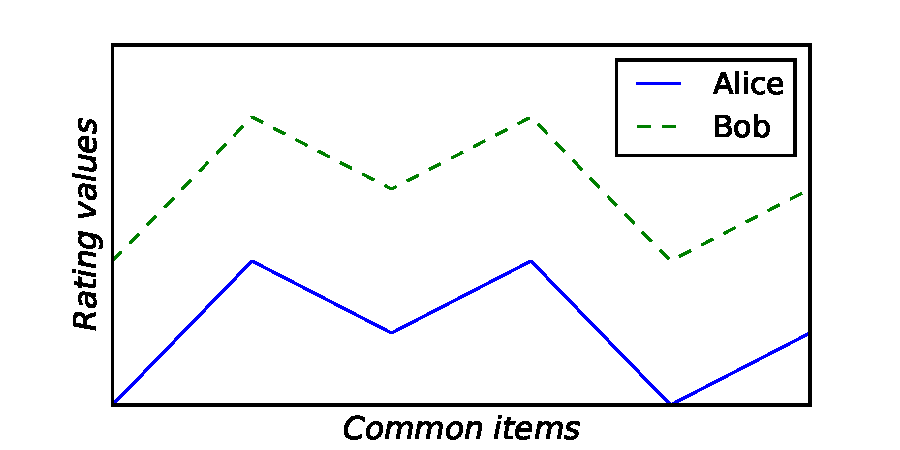
\includegraphics[width=4in]{figures/clones.pdf}
\caption{Bob is a perfect clone of Alice, and Alice is a perfect clone of Bob.}
\label{FIG:alice_and_bob_clones}
\end{figure}

It is obvious that in collaborative filtering, clones are of great interest
when it comes to predicting a user's ratings, and yet the information they provide
is often discarded. Indeed, in Figure \ref{FIG:alice_and_bob_clones}, Alice and
Bob would definitely not be considered as neighbors, so Bob would not be used to
predict Alice's ratings, and Alice would not be used to predict Bob's ratings.
The principle underlying the analogical clone-based view is the following: for
predicting a missing rating for $u$, we not only look at its nearest neighbors
but also at the users $v$ whose ratings are such that $r_{ui} = r_{vi} + t_{vu}$
where $t_{vu}$ is a more or less constant \textbf{correction term} that can be
either positive or negative. This correction term is the difference between
Bob's ratings and those of Alice. When two users $u$ and $v$ are clones, we can
come back to an analogical proportion-based viewpoint by noticing that we have:
$$r_{ui} : r_{vi} :: r_{uj} : r_{vj},~~ r_{uj} : r_{vj} :: r_{uk} : r_{vk},
\dots$$
where $i, j, k, \cdots$ are the common items rated by $u$ and $v$. The algorithms we
will derive will however be much more efficient than those of the previous
section, because they will not rely on an extensive search of 3-tuples of
users.


\subsection{Two new analogical algorithms}

In the following, $C_i(u)$ will denote the set of users that are clones of
$u$ and that have rated item $i$. From the previous informal definitions, one
can easily derive a very general collaborative filtering framework for
predicting a user's rating by taking into account its clones: $$\predrui =
\aggr{v \in C_i(u)}(r_{vi} + t_{vu}),$$
where $t_{vu}$ is a \textit{correction term} that we need to add to $v$'s
ratings so that they correspond to those of $u$. We clearly have a
generalization of the neighborhood approach defined in Section \ref{SEC:neighborhood_approach},
which could be rewritten as:
$$\predrui = \aggr{\begin{subarray}{l}v \in C_i(u),\\ t_{vu} = 0\end{subarray}}(r_{vi} + t_{vu}).$$

Following this general framework, one can construct a great variety of
algorithms with various level of complexity. In the next subsections, we will
propose a very straightforward algorithm, and a more efficient one.

\subsubsection{A straightforward prediction algorithm}
\label{STRAIGHTFORWARD}

We will here design a very basic clone-based algorithm, to show that even a
basic method can outperform the classical neighborhood approach.

Let us first introduce the notion of $t$-clone. In its most simple form, a
user $v$ can be considered to be a $t$-clone of $u$ if the ratings of $v$
exactly differ from those of $u$ by a constant term $t$:
$$
t\text{-}C(u) \eqdef \Set{v \in U | \forall i \in I_{uv},~ r_{ui} = r_{vi} + t}.
$$
From then on, computing $\predrui$ amounts to finding all the users $v$ that
satisfy this criterion, and computing an aggregation of their ratings for $i$,
which can simply be an average. We implemented this basic algorithm described
by Algorithm \ref{ALGO:bruteforce}, and referred to as \textbf{brute-force}.

 \begin{algorithm}[!ht]
   \caption{A brute-force algorithm for clone-based recommendation.}
       \label{ALGO:bruteforce}
       \begin{algorithmic}

      \STATE {\bf Input}: A set of known ratings $R$, a user $u$, an item
      $i$ such that $r_{ui} \notin R$.
      \STATE {\bf Output}: $\hat{r}_{ui}$, an estimation of $r_{ui}$.

      \STATE {\bf Init}:
      \STATE $C \leftarrow \varnothing$ \quad \quad // list of candidate ratings
      \FORALL{ users $v \in U_i$}
        \FORALL{$t$}
          \IF{$v \in t\text{-Clones}(u)$}
          \STATE $C \gets C \cup \{r_{vi} + t\}$ \quad // add $r_{vi} + t$ as a candidate rating
          \ENDIF
        \ENDFOR
	    \ENDFOR
    \STATE $\hat{r}_{ui} \leftarrow \aggr{c \in C} c$
\end{algorithmic}
\end{algorithm}

Of course, one may want to relax the definition of a $t$-clone, as the current
one is too strict and only very few users will satisfy this criterion. In our
implementation, we chose the following condition:
$$
t\text{-}C(u) \eqdef \Set{v \in U |  \sum_{i \in I_{uv}} |(r_{ui} - r_{vi}) -
t| \leq \mid I_{uv}\mid},$$
which amounts to accept $v$ as a $t$-clone of $u$ if on average, the
difference $|r_{ui} - r_{vi}|$ is equal to $t$ with a margin of $1$.
The values of $t$ clearly depend on the rating scale. The datasets on which we
tested our algorithms use the $[1, 5]$ interval, so possible values for $t$
that we have considered are integer values in $[-4, 4]$.

This is obviously a very rough algorithm, to which one could point out numerous
flaws. The first obvious one is its time complexity which is very high, but the
purpose of this brute-force algorithm is simply to show that even such a basic
clone-based approach can lead to better results than a basic neighborhood
method, as we will see in the experiments section.

\subsubsection{Modeling clones with the similarity measure}
Another option to consider clones is to use the well known neighborhood-based
formula, and capture their effects using an appropriate similarity measure.
Recall that the general neighborhood formula is as follows:

$$\predrui = \frac{\sum\limits_{v \in N_i^k(u)} r_{vi} \cdot \ssim(u, v)}
{\sum\limits_{v \in N_i^k(u)}\ssim(u, v)}.$$

We have seen that this formula is commonly used with classical similarity
metrics such as Pearson similarity, Cosine similarity, or inverse of MSD.
However, these similarities are not fully satisfactory when it comes to
clones. Indeed with these metrics, two users are considered to be close if
their common ratings are often the same, but two perfect clones $u$ and $v$
with a significant correction term $t_{vu}$ would be considered as being far from
each other, thus involving a loss of information.

We propose the following simple choice of metric to measure how two users
relate as clones:
$$\clonedist(u, v) \eqdef  \frac{1}{\mid I_{uv} \mid} \cdot
\sum\limits_{i \in I_{uv}} \left[(r_{ui} - r_{vi}) - \mu_{uv}\right]^2,$$
where $\mu_{vu}$ is the mean difference between ratings of $u$ and $v$:
$$\mu_{uv} \eqdef \frac{1}{\mid I_{uv}\mid}\sum_{i \in I_{uv}} (r_{ui} -
r_{vi}).$$

We can understand this distance in two ways:
\begin{itemize}
\item it can be regarded as the variance of the difference of ratings between
  $u$ and $v$,
\item or it can be regarded as a simple MSD measure (defined in Section
  \ref{SEC:neighborhood_approach}) to which the mean difference of ratings between $u$ and $v$ has
    been subtracted.
  \end{itemize}

As our measure $\clonedist$ is a distance, it needs to be turned into 
a similarity measure. A common choice is to take its inverse (while accounting
for zero division):
$$\clonesim(u, v) = \frac{1}{\clonedist(u, v) + 1}.$$

\noindent
Once we know how to find the clones of a user, it is easy to output
a prediction using the classical neighborhood approach:
$$\predrui = \frac{\sum_{v \in N_i^k(u)} (r_{vi} + \mu_{uv}) \cdot \clonesim(u,
v)}{\sum_{v \in N_i^k(u)} \clonesim(u, v)}.$$

This algorithm will be referred to as \textbf{Clone}. For the sake of completeness, we
also tried the same formula but with a more basic similarity metric that does
not care about clones: MSD.

\subsection{Current advances in neighborhood-based techniques}
\label{SEC:current_advances_neighborhood_techniques}

What we have seen so far in terms of neighborhood methods are the rough, basic
techniques that have existed for a long time. Actually, more sophisticated
approaches have been developed, in particular during the Netflix competition.
The one we will describe here has been popularized in \cite{BelKorSIGKDD2007},
and makes use of \textbf{baseline predictors}:
$$\predrui = b_{ui} + \frac{\sum\limits_{v \in N_i^k(u)} (r_{vi} - b_{vi})
\cdot \ssim(u, v)} {\sum\limits_{v \in N_i^k(u)}\ssim(u, v)},$$
where $b_{ui}$ is a baseline (or bias) related to user $u$ and item $i$. Its
expression is $b_{ui} = \mu + b_u + b_i$, where $b_u$ is supposed to model how
$u$ tends to give higher (or lower) ratings than the average of all ratings
$\mu$, and $b_i$ is supposed to model how $i$ tends to be rated higher or lower
than $\mu$. For example, if the mean of all ratings is $\mu = 3$, and the
ratings of a user are $(2, 2, 1)$, its bias $b_u$ would be close to $-1$.

Baselines are computed by solving a regularized least squares problem:
$$\min_{b_u, b_i} \sum_{r_{ui} \in R} \left[r_{ui} - (\mu + b_u + b_i)\right]^2
+ \lambda \left(b_u^2 + b_i^2 \right),$$
which can be achieved efficiently by stochastic gradient descent, or
alternating least squares. The regularization terms are here to avoid
overfitting: they allow to give more confidence to biases that are computed on
a high number of ratings. In our previous example, the user had only rated $3$
items so we cannot reliably say that its real bias is close to $-1$.
The regularization term will allow to give a value closer to 0 for this user
bias.

As a side note, notice that this optimization problem has the same look as the
one we used for the PMF algorithm of Section \ref{SEC:matrix_facto}. In fact, the use of
baselines can be easily combined with the matrix factorization model, leading
to the following optimization problem:
$$\min_{b_u, b_i, p_u, q_i} \sum_{r_{ui} \in R} \left[r_{ui} - \predrui\right]^2
+ \lambda \left(\norm{}{q_i}^2 + \norm{}{p_u}^2 + b_u^2 + b_i^2 \right),$$
with $\predrui = \mu + b_u + b_i + q_i^tp_u$. This prediction algorithm is
called SVD \cite{KorBel11}, and is nothing but the PMF algorithm with user and
items biases. Its extension to handling implicit ratings is called SVD++
\cite{KorBel11}, but we will not describe it here.

In their work, the authors have used this particular similarity metric, that is
in perfect accordance with their prediction formula:
$$\text{sim}(u, v) = \frac
{ \sum\limits_{i \in I_{uv}} (r_{ui} -  b_{ui}) \cdot (r_{vi} - b_{vi})}
{\sqrt{\sum\limits_{i \in I_{uv}} (r_{ui} -  b_{ui})^2} \cdot
\sqrt{\sum\limits_{i \in I_{uv}} (r_{vi} -  b_{vi})^2}}.$$

It is simply a Pearson correlation coefficient, except that instead of
centering ratings with their averages, they are centered with the baseline
predictors. This seemingly simple tweak actually has various consequences that
are very interesting. An intuitive and illuminating way to look at this
algorithm as a whole is to see that it conceptually follows these steps:
\begin{enumerate}
  \item Compute $R'$, the set of all ratings normalized by the corresponding
    baselines: $r'_{ui} = r_{ui} - b_{ui}$.  $R'$ can be regarded as the set
    where all ratings are given from the same frame of reference (in this case
    $0$), thus
    discarding any bias coming from the users or from the items. In $R'$,
    ratings can then be considered as absolute, in the sense that they are not
    spoiled by the users' moods or the items inherent popularity.
  \item Using $R'$, compute similarities between users using the Cosine
    similarity (the Cosine similarity is the same as the Pearson correlation
    coefficient, except that quantities are not centered).
  \item Output a prediction using the basic neighborhood formula. As this
    prediction belongs to the same space of $R'$ where ratings have no bias, it
    needs to be transposed back to the space of $R$ for performance evaluation
    purposes. This is why $b_{ui}$ and $b_{vi}$ are added (or subtracted) in
    the prediction formula of $\predrui$.
\end{enumerate}
\noindent
In what follows, this algorithm will be referred to as $\knns$.

\noindent
It is very clear that the use of the baseline predictors and the use of
clone-based recommendation are motivated by the same reason: they both come
from the fact that users (and items) tend to interpret the rating scale
differently.  This means that $\knns$ implicitly takes the idea of clones into
account, and thus a form of analogical reasoning.  Differences and resemblances
of these two approaches will be discussed in the next section.

\subsection{Experiments and discussion}
\label{SEC:experiments_clone}

To assess the suitability of our clone-based view of recommendation, we have
evaluated the accuracy of the brute-force and Clone algorithms, and compared
them to the previously mentioned approaches: the basic neighborhood method
($k$-NN), and
the neighborhood method taking into account user and item biases ($\knns$). For
reasons that will become clear at the end of this discussion, we also evaluated
the Bsl algorithm, whose prediction is simply the baseline predictor, i.e.
$\predrui = b_{ui}$. The evaluation protocol is the same as that of Section
\ref{SEC:experiments_analogical_reco_basic}, i.e. results are averaged over a 5-folds cross-validation
procedure. In addition to the MovieLens-100k dataset presented earlier, we also
used the MovieLens-1M dataset containing 1 million ratings with 6000 users and
4000 movies.  For each of these algorithms, the number of neighbors or clones
used to output a prediction is $k = 40$, except for the brute-force algorithm
where the number of clones cannot be controlled. The RMSE and MAE of the
algorithms are reported on Table
\ref{TAB:clone_based_rmse_mae}.

\begin{table}[ht]
  \centering
  \begin{tabular}{ l  l  l  l  l l l }
\toprule
    & & &  \multicolumn{2}{ c }{ML-100k}  & \multicolumn{2}{ c }{ML-1M} \\
  \cmidrule(lr){4-5}
  \cmidrule(lr){6-7}
    Algorithm& Details  & & RMSE & MAE  & RMSE & MAE \\
\midrule
    $k$-NN & MSD & $k=40$&  .979 & .773 & .921 & .725\\
    Brute-Force &  & & .948 & .737 & & \\
  \cmidrule(lr){1-2}
    \multirow{2}{*}{Clone} & \clonesim & $k=40$& .936 & .733 & .899& .705\\
                           & MSD & $k=40$ &  .931 &  .732 & .897 &  .707\\
  \cmidrule(lr){1-2}
    $\knns$ & & $k=40$ & .921 & .721 & .869& .680\\
    Bsl & &  & .945 & .749 & .909& .719\\
\bottomrule
\end{tabular}
  \caption{RMSE and MAE of our clone-based algorithms on the MovieLens-100k and
  1M datasets.}
  \label{TAB:clone_based_rmse_mae}
\end{table}

It is very clear that even a very straightforward approach of the clone-based
recommendation principle significantly outperforms the most basic $k$-NN
algorithm, and thus validates the need to take into account biases between
users. The brute-force is however a lot heavier to compute, and thus not very
suitable for real world recommendation purposes (its performances on the
MovieLens-1M dataset simply could not be computed). The two other clone-based
algorithms, however, have the exact same complexity of any $k$-NN-based
algorithm, which is a significant improvement from the algorithm described in
Section \ref{SEC:analogical_reco_basic_algo}.\\

Our two Clone algorithms output (almost) exactly the same
accuracies. This may seem a bit surprising, because the Clone MSD algorithm
does not take into account clones in the similarity measure, and we would
expect it to yield a lower accuracy. But this result still gives a further
reason to consider clones as useful predictors: the only difference between the
Clone MSD algorithm and the $k$-NN MSD algorithm (whose accuracy is much worse)
is that in the prediction of Clone MSD, the mean differences $\mu_{uv}$ between
the ratings of $u$ and its neighbors are taken into account. If this
(seemingly) simple change can make such a significant difference in the
accuracies, this means that the way users relate as clones is an important
feature of the dataset and should not be ignored.

Performances of the Clone algorithms are close to those of the state of the
art $\knns$ algorithm, yet the difference is more striking on the MovieLens-1M
dataset. It is however important to understand that these algorithms differ on
the following points:
\begin{itemize}
\item The Clone algorithms do not address item bias, which is a significant
  drawback. It is not unreasonable to believe that incorporating item bias
  in the prediction would lead to better results.
\item There is a subtle yet meaningful difference of interpretation between the
  biases induced by both algorithms. In the Clone algorithm, biases are all
  pairwise, meaning that they involve two users, and they are computed on items
  that both users have rated. As for the $\knns$ algorithm, there is no such
  thing as a pairwise bias. Bias for a given user is computed using only its
  own ratings, and is a result of a global optimization problem involving the
  global mean of all ratings, which means that every single rating in $R$ has
  an impact on the bias. As baselines are computed on the whole training set,
    they tend to capture most of the noise when the training set gets bigger.
    This may explain why the difference between the Clone algorithms and
    $\knns$ is more striking on the MovieLens-1M dataset.
\end{itemize}

As previously mentioned in Section \ref{SEC:similarity_measures}, it is recommended to perform a
shrinkage on the similarity measure of algorithm $\knns$, in order to take into
account the number of common items between two users: the more items they
share, the more confident we are when computing their similarity
\cite{KorACM2010}. Such techniques can further improve both RMSE and MAE of the
algorithm.  Similarly, in the clone-based approach, it might be of interest to
discount clones that rely on a too small number of common items.\\

Leaving clones for a moment, let us focus now on the Bsl predictor. Bsl outperforms by far the RMSE of the
$k$-NN algorithm, and in fact if we go back to table
\ref{TAB:parall_performances_comparison} on page
\pageref{TAB:parall_performances_comparison}, we see that it outperforms also the
algorithms mentioned there. Yet, this algorithm is unable to output
personalized recommendations: all the recommendations would be the same for
\textbf{any} user! This is simply due to the fact that in the prediction
$\predrui = \mu  + b_u + b_i$, the only user-dependent factor is the term
$b_u$, which is the \textbf{same} in all the predictions regardless of the
item. The point of this remark is to exhibit one of the drawbacks of RMSE that
we already mentioned before: RMSE is not an appropriate measure when it comes
to assess user-system interactions.

Indeed, what ultimately matters is how well a recommender system can
\textbf{rank} the preferences of a user for all the items. Also, rather than
defining clones with the general numerical criterion ($r_{ui} = r_{vi} +
t_{vu}$), we may instead consider that two users are clones if they order their
common items in the same way. Back to Figure \ref{FIG:alice_and_bob_clones}, we
see that Alice and Bob are perfect clones and we actually do not need to know
the real rating values: only the order matters. The goal of the next section is
precisely to investigate this ordinal view of ratings, and to see how it can be
embedded in our clone-based framework.

\subsection{Towards an ordinal view of ratings}

We will here investigate if we can devise a counterpart of the numerical clone-based
approach, which would be compatible with an ordinal view of the ratings.
Indeed, an extreme way for unbiasing and comparing two sets of ratings is to
forget about their numerical values, and only consider their respective rankings. The
idea of viewing ratings in a ordinal manner is not new, and has been advocated
for example in \cite{KorSillRECSYS11}.  In this section, we will discuss an
ordinal counterpart of the analogical approach previously presented.
Analogical reasoning with ordinal data has first been proposed in
\cite{MicBarCAP09}, yet with a different concern.

\subsubsection{An algorithm for rank prediction}
Indeed, the idea that ``\textit{the rating of user $u$ for item $i$ is to the
rating of user $v$ for item $i$ as the rating of user $u$ for item $j$ is to
the rating of user $v$ for item $j$}'' may be understood  as well in an ordinal
manner. This leads to state that ``\textit{the relative ranking of item $i$
  among the ratings given by user $u$  is to the relative ranking of item $i$
  among the ratings given by user $v$ as the relative ranking of item $j$ among
  the ratings given by user $u$  is to the relative ranking of item $j$ among
the ratings given by user $v$}''.

This means that we need to compare the rankings given by two users $u$ and $v$
on their common items. In the following, $\rho_{ui}$ denotes the relative
ranking of item $i$ out of all the items rated by $u$. Our goal is to estimate
all values of $\rho_{ui}$, for any user and any item. The main steps of a
possible algorithm would be as follows:
\begin{enumerate}
  \item Compute similarities between users, based on their rankings. A very
    popular similarity ranking measure is the Spearman's rank correlation
    coefficient (or Spearman's rho), that will be described later.
  \item Compute an estimated rank $\hat{\rho}_{ui}$ as an aggregation of all the
    rankings $\rho_{vi}$ extracted from the $k$ nearest neighbors (using
    Spearman's rho as similarity):
    $$\hat{\rho}_{ui} = \frac{\sum\limits_{v \in N_i^k(u)} \rho_{vi} \cdot
    \ssim(u, v)}{\sum\limits_{v \in N_i^k(u)} \ssim(u, v)}.$$
\end{enumerate}

This is obviously very similar to the numerical clone-based approach described
before, but instead of predicting a rating, we output the prediction of a rank. This
approach is denoted as \textbf{RankAnlg}.

The computation of Spearman's rho takes into account the relative rankings of
the ratings, and is computed as follows:
$$
\text{Spearman}(u, v) \eqdef \frac{\mathop{\text{Cov}}\limits_{i \in I_{uv}}(\rho_{ui},
\rho_{vi})}{\mathop{\text{std}}\limits_{i \in I_{uv}}(\rho_{ui}) \cdot
\mathop{\text{std}}\limits_{i \in
I_{uv}}(\rho_{vi})},
$$
where Cov naturally stands for covariance and std is the standard deviation.
Spearman's rho is usually defined as a statistic for random variables, and we
here have translated it as a realization of this statistic in our
recommendation setting. A common issue when dealing with rankings is that there
may be ties in the data. Consider for example user $u$ from Table
\ref{TAB:rankings}, whose ratings are $1, 1, 2, 3, 3, 3$ for items $i_1, i_2,
i_3, i_4, i_5$ and $i_6$.
\begin{table}[h!]
\centering
  \begin{tabular}{ l  l  l  l  l  l  l }
\toprule
    & $i_1$ & $i_2$ & $i_3$ & $i_4$ & $i_5$ & $i_6$\\
  \midrule
    $r_{ui}$ & 1 & 1 & 2 & 3 & 3 & 3\\
    Raw rankings & 1 & 2 & 3 & 4 & 5 & 6 \\
    Processed rankings $\rho_{ui}$ & 1.5 & 1.5 & 3 & 5 & 5 & 5 \\
\bottomrule
\end{tabular}
  \caption{Values of $\rho_{ui}$ for the user $u$.}
\label{TAB:rankings}
\end{table}
As $i_1$ and $i_2$ have the same ratings, there is no reason to rank $i_1$
before $i_2$, or $i_2$ before $i_1$. The same goes for $i_4, i_5$ and $i_6$,
and this is why the first ranking option (raw rankings) is not a suitable one.
Instead, it is common to consider that the ranking of a given item is the mean
of the raw rankings for the items that share the same rating value. In our case,
$\rho_{u{i_1}} = \rho_{u{i_2}} = \frac{1 + 2}{2}$, and $ \rho_{u{i_4}} =
\rho_{u{i_5}} =  \rho_{u{i_6}} = \frac{4 + 5 + 6}{3}$.
This process leads to a better estimation of Spearman's rho, and is equivalent
to averaging over all possible permutations between the raw ranks of items with
equal ratings.



\subsubsection{Experiments}

We evaluated the performance of our algorithm and compared it to other
previously described approaches, using the exact same evaluation protocol as in
the previous sections. The MovieLens-1M dataset was not benchmarked, because
the computation of Spearman's rho was too computationally intensive on this
bigger dataset.

RMSE and MAE are good measure for evaluation rating prediction accuracy, but
are not suitable when it comes to evaluate rankings. A better measure is the
Fraction of Concordant Pairs (FCP), which evaluates the probability that given any two
items $i$ and $j$ rated by any user $u$, the system has correctly estimated
whether $u$ prefers $i$ over $j$, or the reverse. To compute the FCP, we need to
use intermediate measures. Following the notation of \cite{KorSillRECSYS11},
$c_u$ defines the number of concordant pairs for user $u$, and $d_u$ is the
number of discordant pairs. The FCP is then computed over all users as the
proportion of concordant pairs.

\begin{align*}
  c_u &\eqdef \Big| \Set{(i, j) \in I^2 \quad | \quad \predrui > \predruj \text{ and
  } r_{ui} > r_{uj}}\Big|,\\
  d_u &\eqdef \Big| \Set{(i, j) \in I^2 \quad | \quad \predrui \geq \predruj \text{
    and } r_{ui} < r_{uj}}\Big|,\\
  \FCP &\eqdef \frac{\sum\limits_{u \in U} c_u}{\sum\limits_{u \in U} c_u +
  \sum\limits_{u \in U} d_u}.
\end{align*}
Here, $\predrui$ may represent either a rating prediction or a ranking
prediction $\hat{\rho}_{ui}$.

Results are reported in table \ref{table:res100kRank}.
\begin{table}[!ht]
\centering
\begin{tabular}{ l l  l l }
\toprule
     & RankAnlg &  $k$-NN & $\knns$\\
\midrule
\FCP  &  .7063   & .7096 &  .7163   \\
\bottomrule
\end{tabular}
\caption{\FCP~ of our rank prediction algorithm on the MovieLens-100k
  dataset.}
\label{table:res100kRank}
\end{table}
Unfortunately, even a basic algorithm such as $k$-NN that was not designed for ranking
prediction performs better in terms of FCP. To explain this difference, one may
look at the distribution of average support over all the predictions, as shown
on figure \ref{FIG:support_spearman_MSD}. Between
two users $u$ and $v$, the support is defined as the number of common items
$|I_{uv}|$ which was used to compute the similarity between $u$ and $v$. For
a given prediction $\predrui$, the average support is the average of all the
supports $|I_{uv}|$ over all users $v \in N_i^k(u)$.

\begin{figure}[!h]
\centering
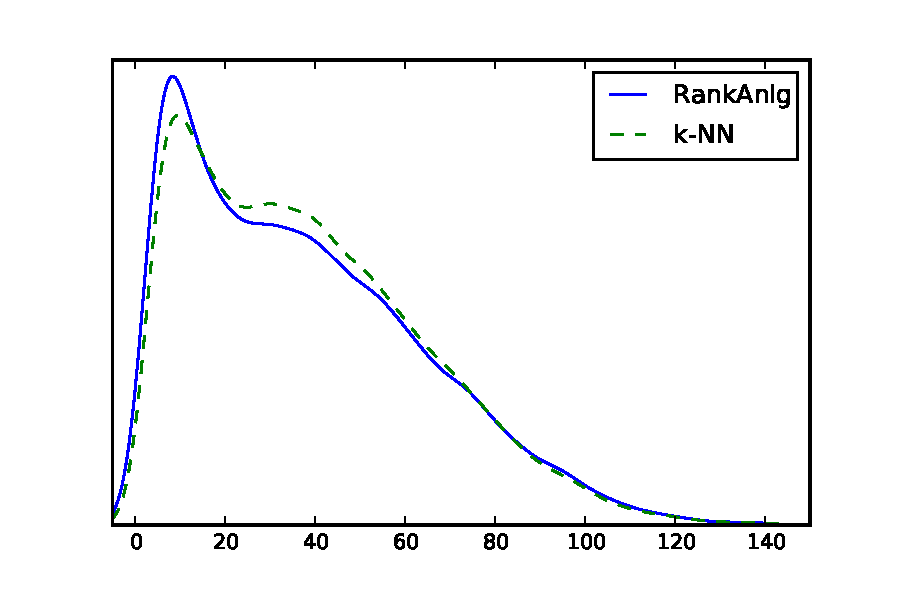
\includegraphics[width=2.5in]{figures/support.pdf}
  \caption{Distribution of average support for Spearman's rho (RankAnlg) and
  MSD ($k$-NN).}
\label{FIG:support_spearman_MSD}
\end{figure}

The use of Spearman's rho tends to provide with neighbors that have smaller
support values, thus leading to a less significant and less accurate estimation
of the neighborhood, which may explain the differences in performance.

This closes for now our contributions to analogical recommendation. We will
come back to it in the conclusion of this chapter, and we will now focus on a
somewhat unrelated problem: analogical proportion mining in databases. As we
will see though, analogical recommendation can in fact be viewed as both a
motivation \textbf{and} a purpose for the mining of analogical proportions.

\section{Mining analogical proportions}
\label{SEC:mining_analogical_proportions}

Let us recap a bit the first section of this chapter, where we described our
first attempt to design an analogical-based recommendation algorithm. As it is
a direct application of the analogical inference principle, our algorithm
suffers from the same drawbacks as the conservative and extended learners
introduced in Chapter \ref{CHAP:functional_definition}: the time complexity is
cubic, which makes it impossible to use in actual systems and hard to evaluate
accurately. Also, the performances of this algorithm were quite modest, even in
its most elaborated forms.

Our analogical inference principle used in the first section states that if
four users $a, b, c, d$ are in analogy, then their ratings for an item $i$ that
$d$ has not rated should also be in analogy:
$$
\inferrule{r_{aj} : r_{bj} :: r_{cj} : r_{dj} ~~ \forall j \in
I_a \cap I_b \cap I_c \cap  I_d}
{r_{ai} : r_{bi} :: r_{ci} : r_{di} ~~ \forall i \in I_a \cap I_b \cap I_c,
\text{ and } i\notin I_d }
$$
But we have so far neglected a central question: do such proportions actually
exist in our database? Can we find enough 4-tuples of users such that their
common ratings are in proportion? And if we can, how good are these proportions? We already
acknowledged that absolutely perfect proportions are actually hard to find, and
this is why we have relaxed the condition for an analogy to hold in Algorithm
\ref{ALGO:analogical_recommendation}.

In this section, we will design an algorithm that is able to answer all of
the above questions, by extracting all the analogical proportions underlying a
database that satisfy some given quality criterion. We will apply this algorithm
to the MovieLens database, and see how this relates to our recommendation task.
We will here look for analogies between items (movies in our case) instead of
looking for analogies between users, because the interpretation of a
movie-based proportion is actually easier, and because the parallel with
association rules (described below) will be more natural. Both problems are
symmetric though, and our solution can be adapted to user proportions in a
straightforward manner.

Because our method for mining analogical proportions is inspired from the mining
of association rules, we will first review this topic in the next subsection.

\subsection{Association rules}

Association rules are pieces of information that one can extract from a
database, and that reveal dependencies between items. Recommendation is one of
the principal application of association rules. Starting from the association
rule $i \implies j$, which means that users that buy $i$ tend to buy $j$ with
high probability, a recommendation system can suggest $j$ as soon as we bought
$i$ (but not yet $j$). A well-known example of association rule is the famous
$\text{beer} \implies \text{diapers}$ association, which was revealed after
mining association rules in a supermarket selling history, suggesting that
people tend to buy beer and diapers altogether. We now formally introduce the
problem of \textbf{association rule mining}.

Let $I = \Set{i_1, i_2, ..., i_m}$ be a set of $m$ items, and let $T =
\Set{t_1, t_2, ..., t_n}$ be a multiset of transactions, where each transaction
is a subset of $I$: $\forall i, ~ t_i \subseteq I$. A transaction simply is a set of items
that are purchased together. An association rule is expressed in the form $ X
\implies
Y$, where $ X \subsetneq I, ~ Y \subsetneq I$, and $X \cap Y = \varnothing$. $X$ and
$ Y $ are sets of items that we will call \textbf {itemsets}, and usually $Y$
is restricted to a single item. We define the \textbf{support} $\supp (X) $ of
an itemset $X$ as the proportion of transactions that contain it:
$$\supp(X) \eqdef \frac{\mid \Set{t \in T | X \subseteq t}\mid}{\mid T \mid}.$$
Sometimes, the support is not defined as a proportion but rather as the
absolute number $\mid \Set{t \in T | X \subseteq t}\mid$. Various
measures can be used to evaluate the quality of an association rule, such as
the \textbf{confidence} which can be expressed as:
$$\text{Conf}(X \implies Y)~\eqdef~\frac{\supp (X \cup Y)}{\supp (X)}.$$
As could be naturally expected, $\text{Conf}(X \implies Y)$ is equal to $1$
when the items of $X$ and $Y$ are systematically bought together, and decreases
if the set $X$ is sometimes found in a transaction that does not contain $Y$.

The mining of association rules is a popular research topic, and has been
extensively studied. In a perfect world with unlimited computational resources,
a naive association rules mining algorithm would be as follows:
\begin{enumerate}
\item First, generate the power set of $I$, i.e. the set of all subsets of $I$
  that we denote $2^I$.  We know that the elements in $2^I$ are partially
  ordered with respect to inclusion, and $2^I$ can be represented as a lattice
    where the \textit{join} is the union and the \textit{meet} is the intersection.
\item Let $I_S$ be any of the $2^m$ itemsets in $2^I$. Then for each $I_S$,
  compute all partitions $\set{X, Y}$ of $I_S$ and calculate the confidence
    associated with the rule $X \implies Y$. If the confidence is above a given
    threshold, then keep the association rule, else discard it.
\end{enumerate}

The second step remains reasonable and cannot really be optimized, but the
first one is obviously impossible to perform in practice due to the terrific size of $2^I$,
when real-world databases usually contain hundreds or thousands of items.
The most famous algorithm for association rule mining probably is the
\textbf{Apriori} algorithm introduced in \cite{AgrSriVLDB94}, that we will
briefly review. Using Apriori allows to scan the itemset lattice in an
efficient way, avoiding many useless nodes.

Ultimately, we are only interested in association rules where the support of
the involved itemsets is high. An itemset whose support is above some given
threshold $\alpha$ is called a \textbf{frequent} itemset. The downward-closure
property of support states that if $I_S$ is a frequent itemset, then all of its
subsets are also frequent itemsets. For example, if the itemset
$\Set{\text{apple, banana, orange}}$ is found in more than 30 transactions,
then the three subsets $\Set{\text{apple, banana}}$, $\Set{\text{apple,
orange}}$ and $\Set{\text{banana, orange}}$ must also be found in \textbf{at
least} 30 transactions. Conversely, if the two sets $\Set{\text{kiwi, pear}}$ and
$\Set{\text{kiwi, strawberry}}$ are found in less than $30$ transactions, we
are sure that their union $\Set{\text{kiwi, pear, strawberry}}$ will also be
found in less than $30$ transactions. So if we are only interested in itemsets
whose support is higher than $30$, there is no point in building the set
$\Set{\text{kiwi, pear, strawberry}}$, or any of its supersets.

Taking advantage of this fact, a basic version of the Apriori can be described
in the following steps:
\begin{enumerate}
  \item Consider all itemsets of size $1$ whose support is above $\alpha$.
  \item By joining these $1$-itemsets, build all possible $2$-itemsets and only
    keep those whose support is above $\alpha$.
  \item By joining these $2$-itemsets, build all possible $3$-itemsets and only
    keep those whose support is above $\alpha$.
  \item Repeat the process: all the frequent $k$-itemsets are built by joining
    the frequent $k-1$ itemsets.
  \item Once all the frequent itemsets have been computed, the second step of
    the above naive algorithm is used to assess the confidence of the
    association rules.
\end{enumerate}
In the end, we are provided with a set of association rules than comply with
some quality requirements, and that give us insightful information that link
the elements of our database.

%Sur le mode des proportions analogiques, on admettra que {\it le dentifrice
%est à la brosse à dent ce que le beurre est à la biscotte}.  Dans ce
%cas, on peut penser recommander à quelqu'un ayant acheté dentifrice,
%brosse à dent et beurre, d'acheter des biscottes. Sur quelle base?  Sur la
%base que la relation liant dentifrice et brosse à dent est la même que
%celle liant beurre et biscottes.

Just like association rules, the identification of analogical proportions in a
database is an additional information source, and deserves to be addressed. We
will now get to the heart of the matter.

\subsection{Looking for analogies in an incomplete database}

In order to avoid any ambiguity, we will formally define our problem first.
\subsubsection{Problem definition and links to association rules}

We will be looking for analogies between items in the MovieLens database, but
our method can naturally be extended to any other database with the same
structure.  We dispose of a set of users $U$ and a set of items $I$. Each user
$u$ has rated (or purchased) a given set of movies $I_u \subseteq I$. In this
setting, each user $u$ can be considered as a transaction $t$, as
defined in the previous section. The set of all the ratings $\rui$ is denoted
$R$ and can be viewed as a sparse matrix where users are columns and items are
rows (or the reverse).  For now, we do not care about the rating values and
just focus on whether the rating exists or not (just like we only care about
the fact that an item has been bought in the case of association rules). We
will only make use of the rating values when we will evaluate how good the
proportions are, in later subsections.

We need to insist here on the fact that we are dealing with a \textbf{sparse}
database.  In the case where all values in $R$ are known, the problem of mining
analogical proportion is pretty trivial: all we need is to look for all
$4$-tuples of items, and evaluate how good the proportion $a:b::c:d$ is. This
search is in $\mid I \mid^4$ which is extremely expensive, but there is
probably no shortcut. This problem is not really interesting in the sense that
there is no need to come up with an elaborated algorithm. Its parallel in the
association rules world corresponds to the case where each transaction
$t_i$ contains all the items ($\forall i, t_i = I$): the very idea of
association rule does not make sense anymore. The problem we propose to address
here is different: the matrix $R$ is sparse and the set of users that have
rated (purchased) the items is different each time: for all items $i$ and $j$
(or at least for most), we have $U_i \neq U_j$. We thus cannot just look at all
$4$-tuples of items and check if they are in analogy. Or more accurately we
could, but as we are ultimately interested in good analogies (i.e. analogies
involving a sufficient number of ratings), we can make use of the
downward-closure property just like the Apriori algorithm, which will allow us
to avoid many $4$-tuples that could not lead to good analogies.

Let's now consider four users $a, b, c, d$, and our task is to find out if
these four users make up a valid analogy. For now, we do not know in which
order we need to consider them.  Just like for association rules, the notion of
support still makes sense here because these four users make up a $4$-itemset:
$$\supp(a, b, c, d) \eqdef \frac{\mid I_{abcd}\mid}{\mid I\mid},$$
where $I_{abcd}$ is the set of items that $a, b, c$ and $d$ have all rated.
Here again, we will only be interested in proportions whose support is greater
than some threshold $\alpha$: a proportion built on only two components is a
lot less meaningful than a proportion built on dozens of components.

When given four items $a, b, c, d$, the question is now to find out which is
the proportion that actually holds. It could be $a:b::c:d$, but it could just
as well be $a:b::d:c$ or $a:c::d:b$, or any of the $24$ ($4!$) combinations of
these four elements. Fortunately, we do not have to test all the $24$
orderings.  We know from Chapter \ref{CHAP:formal_analogical_proportions} that
there are exactly 3 equivalent classes of analogies, which are represented by:
\begin{itemize}
  \item $a:b::c:d$,
  \item $a:b::d:c$,
  \item $a:d::c:b$.
\end{itemize}
Thus, testing these three orderings is enough to find out about the $24$
possible forms of analogies. To assess the quality of a proportion, we will
use a function $f$ that plays a similar role to the confidence function for
association rules. Then, it will be natural to only consider analogies that
are above some given quality threshold. Simply put, we would consider
$a:b::c:d$ as a valid analogy if $f(a:b::c:d) \geq \beta$. In the end we are
left with a set of proportions that represent analogical relations between four
items.

\subsubsection{Assessing the quality of a proportion}

We will here describe various functions $f$ that can assess the quality of a
proportion. The four items $a, b, c, d$ are considered as vectors of ratings in
the space of their common users,
and we will consider two cases: that of the binary rating scale $[0, 1]$, and
that of the gradual rating scale $[1, 5]$. Note that here, in case of the
binary rating scale, the value $1$ is associated with \textit{like} and the
value $0$ is associated with \textit{dislike}, but a value of $0$
\textbf{still} means that the user $u$ has rated the item $i$. In some
settings (e.g. with the unary rating scale), a value of $0$ can be interpreted
as the absence of rating, but this view is not compatible with our problem: if
$\rui = 0$ means $\rui \notin R$, the four items $a, b, c, d$ would only be
represented as vectors of constant value $1$, where analogies are all trivial
because their only pattern is $1:1::1:1$. Instead, when $0$ still means that
the user has rated the item, the items can be represented as Boolean vectors,
which is fortunate because we know how to deal with Boolean proportions.

Naturally, the quality functions that we can define will depend on the nature
of the rating scale.

\begin{itemize}
  \item When we have a binary rating scale, the obvious choice for assessing
    the quality (or rather the \textit{badness}) of a proportion is the
    analogical dissimilarity defined in Section \ref{SEC:extended_classifier}. For Boolean
    vectors, the analogical dissimilarity is defined as the number of
    components that need to change in order to have a perfect proportion. Note
    however that we ultimately want to \textbf{compare} the quality of
    different proportions, and the fact is that no two $4$-tuples of items will
    have the same common users, so the item vectors of the two different
    $4$-tuples will likely have different dimensions. Therefore, it might be
    wise to consider the \textbf{relative} analogical dissimilarity, which is
    the classical AD divided by the dimension of the vectors.
  \item Another obvious quality measure in $\mathbb{B}^m$ simply is the number
    of components where a Boolean proportion perfectly holds. It is a slightly
    less conservative approach than the above one but still very similar. In
    practice, this means that the two proportions $0:1::1:0$ and $1:0::0:1$
    will be given an AD of $1$ instead of $2$. Here again, considering a
    fraction rather than an absolute number may be more meaningful, because
    of the different dimensions.
  \item When the rating scale is numerical (e.g. $[1, 5]$), the analogical dissimilarity is
    defined as $\norm{p}{(a - b) - (c - d)}$, and indicates how well the
    parallelogram $abcd$ holds. Clearly, this can also be used as a measure of
    quality of the proportion.
  \item Another option for the gradual rating scale is to use the definitions
    of the fuzzy analogy evaluation described at the end of Section
    \ref{SEC:formal_definitions_proportions}. As the quality of each proportion is
    evaluated in a component-wise fashion, we can choose various aggregation
    functions to assess the overall quality: mean, max, min, or also compare
    two proportions by lexicographic order. We will give further details in the
    experiments section.
  \item Finally, by adopting a statistical point of view, we can try to
    evaluate the probability of observing the proportion $a:b::c:d$, and
    consider it a meaningful proportion if it is unlikely that we could have
    observed this proportion by random chance alone. This method is highly
    linked to statistical test theory.
\end{itemize}

\subsubsection{Algorithm}

Our algorithm for mining analogical proportions imitates an association rule
mining process: we preliminarily set a threshold $\alpha$ for the support, and a
quality evaluation $f$ along with a threshold $\beta$.

After having built all the $4$-itemsets whose support is above the threshold
$\alpha$ with the Apriori algorithm, we compute the quality of the proportions
associated with the three equivalent classes, and keep those that satisfy our
criterion. These steps are described in Algorithm \ref{ALGO:proportion_mining}.

 \begin{algorithm}[!ht]
   \caption{Analogical proportion mining.}
       \label{ALGO:proportion_mining}
       \begin{algorithmic}

      \STATE {\bf Input}: A set of known ratings $R$, a quality function $f$,
         and two thresholds $\alpha$ and $\beta$.
         \STATE {\bf Output}: A set $\mathcal{P}$ of analogical proportions
         between items.
         \STATE $\mathcal{P} \leftarrow \varnothing$
         \STATE \textit{Candidate retrieval:}
      \STATE Using Apriori, derive all the $4$-itemsets whose support is
         greater than $\alpha$.
         \STATE \textit{Quality evaluation:}
         \FORALL{$(a, b, c, d)$ in the set of $4$-itemsets}
         \FORALL {prop $\in \Set{(a:b::c:d), (a:b::d:c), (a:d::c:b)}$}
         \IF{$f(\text{prop)} \geq \beta$}
         \STATE $\mathcal{P} \leftarrow \mathcal{P} \cup \Set{\text{prop}}$
         \ENDIF
         \ENDFOR
         \ENDFOR
\end{algorithmic}
\end{algorithm}

In theory, it is possible to end up with two non-equivalent proportions in
$\mathcal{P}$ that still relate to the same four items, i.e. we could find in
$\mathcal{P}$ the proportion $a:b::c:d$ as well as the non-equivalent
proportion $a:b::d:c$. It should not seem natural to have these two proportions
in $\mathcal{P}$, so if this happens, it is probably because the quality
function $f$ is too permissive or because the threshold $\beta$ is not
correctly tuned.

We also want to stress the point that the actual rating values are only used in
the second part of the algorithm, i.e. when we evaluate the quality of the
proportions. In the first part involving the Apriori algorithm, the only
information that matter are that a rating exists. Its value is not taken into
account.

\subsection{Experiments and discussion}

As previously indicated, we have considered the MovieLens-100k dataset for our experiments: 100,000
ratings in $[1, 5]$ from $1000$ users and $1700$ movies. We will first treat
ratings as numerical values, and in the second part of this investigation
we will binarize them.

\subsubsection{Numerical ratings}

For our purpose, we actually do not need to set a quality threshold $\beta$,
which would by the way be quite arbitrary. Instead, we will only be interested
in \textbf{comparing} the quality of the  proportions. We will not make use of
the analogical dissimilarity because the AD is dependent on the dimensions of
the vectors, and we will necessarily compare proportions that have different
dimension so this would not make sense. Instead, we have chosen to
compare two proportions by first computing the truth value of each of their
component-wise proportions using the graded-view of analogical proportions
described in Section \ref{SEC:formal_definitions_proportions}, and then by
comparing these truth values in lexicographic order. This allows to compare
proportions that have different dimensions in a more meaningful way.

This fuzzy view of analogical proportion is recalled here: for four real
elements $a, b, c, d \in [0, 1]$, the quality of the analogical proportion
$a:b::c:d$ is evaluated by:
\begin{align*}
A(a, b, c, d) =
\begin{cases}
  1 - |(a - b) - (c - d)| &\text{ if } a \geq b \text { and } c \geq d, \text{
    or } a \leq b \text{ and } c \leq d\\
  1 - \max(|a - b|, |c - d|) &\text{ if } a \geq b \text { and } c \leq d, \text{
    or } a \leq b \text{ and } c \geq d.
\end{cases}
\end{align*}

\begin{testexample}
Consider for example the two $4$-itemsets of Table
\ref{TAB:lexicographic_order}, where ratings $[1, 2, 3, 4, 5]$ have been mapped
to $[0, .25, .5, .75, 1]$. We will consider that the first $4$-tuple $i_1, i_2,
i_3, i_4$ (on the left) is a better proportion than the second one because
once their truth values are sorted, it is the one that comes first. Had we
chosen to compare them with the mean of the truth values, the best proportion
would have been the second one. In the remaining of this discussion, a
\textbf{component-proportion} will denote a proportion between ratings (for
example the proportion $0:1::0:1$ is the first component-proportion of
$i_1:i_2::i_3:i_4$), and in general a proportion  will refer to an analogy
between items (i.e. it is an aggregation of component-proportions).
\end{testexample}

\begin{table}[h!]
\centering
  \begin{tabular}{ c c  c  c  c }
\toprule
 $i_1 $ & $i_2$ & $i_3$ & $i_4$ & $A$\\
  \midrule
    0 & 1 & 0 & 1 & \textbf{1} \\
    0 & .5 & .25 & .75 & \textbf{1} \\
    1 & .5 & 1 & .25 & \textbf{.75} \\
    0 & .5 & 1 & .25 & \textbf{.25} \\
\bottomrule
\end{tabular}
\quad
  \begin{tabular}{ c c  c  c  c }
\toprule
 $i_5 $ & $i_6$ & $i_7$ & $i_8$ & $A$\\
  \midrule
    0 & 0 & 0 & 0 & \textbf{1} \\
    0 & .25 & 1 & .75 & \textbf{.75} \\
    1 & .5 & 1 & .25 & \textbf{.75} \\
    1 & 1 & 1 & .75 & \textbf{.75} \\
\bottomrule
\end{tabular}

\caption{Two $4$-itemsets and their related proportions, with corresponding
  truth value ($A$).}
\label{TAB:lexicographic_order}
\end{table}

Using this comparison procedure, we have looked for the 10 best proportions
with a minimum support of $200$ common users. The results are reported on Table
\ref{TAB:best_prop_num_basic_200}.
\begin{table}[h!]
\centering
  \begin{tabular}{l l  l  l l}
\toprule
    &\multicolumn{1}{c}{$i_1$}  & \multicolumn{1}{c}{$i_2$} &
    \multicolumn{1}{c}{$i_3$} & \multicolumn{1}{c}{$i_4$}\\
  \midrule
 1&   Star Wars & The Emp. Strikes Back & Raid. of the Lost Ark & Return of the Jedi  \\
 2&   Star Wars & Return of the Jedi & Raid. of the Lost Ark & The Emp. Strikes Back  \\
 3&   Star Wars & The Emp. Strikes Back & Return of the Jedi & Raid. of the Lost Ark  \\
 4&   Star Wars & Raid. of the Lost Ark & Return of the Jedi & I.J. and the Last Crus.  \\
 5&   Star Wars & Return of the Jedi & Raid. of the Lost Ark & The Fugitive  \\
 6&   Star Wars & Raid. of the Lost Ark & Return of the Jedi & Back to the Future  \\
 7&   Star Wars & The Emp. Strikes Back & Raid. of the Lost Ark & I.J. and the Last Crus.  \\
 8&   Star Wars & The Emp. Strikes Back & Return of the Jedi & I.J. and the Last Crus.  \\
 9&   Star Wars & The Emp. Strikes Back & I.J. and the Last Crus. & Return of the Jedi  \\
 10&   Star Wars & Raid. of the Lost Ark & The Emp. Strikes Back & The Fugitive\\
\bottomrule
\end{tabular}
\caption{The ten best item proportions with a support of more than $200$ common
  ratings, using $A$.}
  \label{TAB:best_prop_num_basic_200}
\end{table}

The first obvious observation is that only a few movies (exactly $7$) make up
these 10 proportions. This is not really surprising, as we have set the support
threshold quite high, and only a few movies are rated by more than 200 users.
In fact, we found 331 4-itemsets with more than 200 common users, but they only
contain 37 unique movies. Clearly here the involved movies (Star Wars, Indiana
Jones\dots) are extremely popular, and people tend to give them high ratings.
Using notions introduced in Section
\ref{SEC:current_advances_neighborhood_techniques}, we can say that these
movies have a high item bias $b_i$. To confirm this claim, we can check that in
average, the mean rating of these 7 movies is of 4.09, while the average rating
of all movies is only 3.53.

Some of the analogies are actually quite good though. For example the fourth
one \textit{Star Wars (1977)} is to \textit{Raiders of the Lost Ark (1981)} as
\textit{Return of the Jedi (1983)} is to \textit {Indiana Jones and the Last
Crusade (1989)}, or the seventh one which is similar: \textit{Star Wars (1977)}
is to \textit{The Empire Strikes Back} as \textit{Raiders of the Lost Ark
(1981)} is to \textit{Indiana Jones and the Last Crusade (1989)}

Looking at the first and third proportions, we see that the two forms
$i_1:i_2::i_3:i_4$ and $i_1:i_2::i_4:i_3$ are present in the table. These two
forms are non-equivalent, and it does not seem natural to consider these two
proportions as (almost) equally valid. But this result can be explained by
looking at the actual rating values: a great number of them are of the form
$r:r::r:r$ (where $r$ is usually a high rating, given that these movies are
popular). In the two cases, a switch between $i_3$ and $i_4$ has absolutely no
effect on the truth values of the analogies.

This leads us to another point: all these analogies are, after all, quite
trivial. They all concern quite similar movies. We do not mean to offend any
cinema fan, but we believe it is still fair to say that the differences between
a Star Wars movie and an Indiana Jones movie are quite shallow. And these
similarities are reflected in the ratings, where the most common pattern is
$r:r::r:r$ (or close to it), suggesting that people like all these movies the
same.

To try to discover some more surprising analogies, we basically have two
options. The first one is to tweak a bit our quality function $f$ (and in our
case, our comparison function) by penalizing proportions with the pattern
$r:r::r:r$, or inversely by promoting the proportions $r : r' :: r :r'$ where
$r$ and $r'$ are quite different. The second option is to lower the minimum
support threshold, to allow movies that are rated by a reasonable (and not
necessarily very high) number of users. As we have seen, movies with a very
high number of ratings are likely to lead to trivial proportions precisely
because they are popular, and because people like them all equally well in
general. If we really want to ban popular movies, we can also set a
\textbf{maximum} support threshold. This will also have the benefit to limit
the number of itemsets that we consider, leading to a significant improvement
in computation time. These two options will be explored.

\paragraph{Promoting \textit{disagreement} proportions\\}

Table \ref{TAB:best_prop_num_customTV_200} shows the 10 best proportions with a
minimum support of $200$, with a tweaked comparison function. Here, the truth
value of a component-proportion $r_1 : r_2 :: r_3 : r_4$ is defined by:
$$A'(r_1, r_2, r_3, r_4) = \frac{1}{2} A(r_1, r_2, r_3, r_4) + \frac{1}{4} |r_1
- r_2| + \frac{1}{4} |r_3 - r_4|.$$
We are here promoting proportions where rating values tend to disagree, which
should lead to different proportions from that of Table
\ref{TAB:best_prop_num_basic_200}. Proportions are still compared using the
lexicographic order of all the $A'$ values.
\begin{table}[h!]
\centering
  \begin{tabular}{ l l  l  l l }
\toprule
    & \multicolumn{1}{c}{$i_1$}  & \multicolumn{1}{c}{$i_2$} &
    \multicolumn{1}{c}{$i_3$} & \multicolumn{1}{c}{$i_4$}\\
  \midrule
    1& Star Wars  & Pulp Fiction  & The Empire Strikes Back  & The Fugitive   \\
    2& Star Wars  & Pulp Fiction  & Return of the Jedi  & The Fugitive   \\
    3&Star Wars  & Pulp Fiction  & The Empire Strikes Back  & The Silence of the Lambs   \\
    4&Star Wars  & Twister  & Return of the Jedi  & Independence Day  \\
    5&Star Wars  & Return of the Jedi  & The Silence of the Lambs  & Fargo   \\
    6&Star Wars  & The Terminator  & Return of the Jedi  & Pulp Fiction   \\
    7&Star Wars  & Pulp Fiction  & Return of the Jedi  & The Terminator   \\
    8&Star Wars  & The Fugitive  & The Empire Strikes Back  & The Silence of the Lambs   \\
    9& Star Wars  & Pulp Fiction  & Return of the Jedi  & The Silence of the Lambs   \\
   10&Star Wars  & Pulp Fiction  & Raiders of the Lost Ark  & The Silence of the Lambs   \\
\bottomrule
\end{tabular}
\caption{The ten best item proportions with a support of more than $200$ common
  ratings, using $A'$.}
\label{TAB:best_prop_num_customTV_200}
\end{table}

We still have a lot of Star Wars movies (and a few Indiana Jones), but the
movies seem more diverse: we now have 11 unique movies, instead of just 7
before. 9 of these proportions comply with the pattern \textit{Star Wars
movie} is to \textit{Other Star Wars movie} what \textit{movie A} is to
\textit{movie B}. This suggests that we should find strong links underlying the
connection between \textit{Movie A} and \textit{Movie B}, because the two Star
Wars movies are deeply related. Is \textit{Pulp Fiction} related to \textit{The
Fugitive}? Is \textit{Twister} related to \textit{Independence Day}? Is
\textit{Fargo} related to \textit{The Silence of the Lambs}? We will not
venture to answer these questions, and leave them to the reader's appreciation.
All we can say is that some forms of analogy seem to emerge from their
respective ratings.  One thing we can note however, is that even though all
these movies are very popular just like in Table
\ref{TAB:best_prop_num_basic_200}, their genres are however quite different:
while we have considered Star Wars and Indiana Jones to be of the same kind, we
can fairly claim that a Star Wars movie is very far from Fargo, Pulp Fiction or
The Silence of the Lambs.

\paragraph{Lowering support threshold\\}

Table \ref{TAB:best_prop_num_basic_10_50} illustrates the ten best proportions
we have found after setting the minimum support at 10, and a maximum support at
50. This drastically reduces the number of $4$-tuples that are explored, and
avoids any highly popular movie.
\begin{table}[h!]
\centering
  \begin{tabular}{ l l  l  l l }
\toprule
    &\multicolumn{1}{c}{$i_1$}  & \multicolumn{1}{c}{$i_2$} &
    \multicolumn{1}{c}{$i_3$} & \multicolumn{1}{c}{$i_4$}\\
  \midrule
  1&   To Catch a Thief  & Laura  & Gigi  & An American in Paris  \\
  2&   Nick of Time  & It Could Happen to You  & Milk Money & Only You  \\
  3& To Catch a Thief  & An American in Paris  & Gigi  & Meet John Doe   \\
  4& Dangerous Minds  & Money Train  & Higher Learning  & With Honors   \\
  5& Judge Dredd  & Under Siege 2: Dark Territory  & The Shadow  & Mortal Kombat   \\
  6& Terminal Velocity & Under Siege 2: Dark Territory  & Money Train  & Drop Zone    \\
  7& Judge Dredd  &Under Siege 2: Dark Territory  &  Mortal Kombat  & Coneheads   \\
  8& To Catch a Thief  & An American in Paris  & Gigi  & Laura   \\
  9&  To Catch a Thief  & Meet John Doe  & Gigi  & An American in Paris   \\
 10&   Nick of Time  & It Could Happen to You  & Only You  & Milk Money   \\
\bottomrule
\end{tabular}
  \caption{The ten best item proportions with a support between $10$ and $50$.}
  \label{TAB:best_prop_num_basic_10_50}
\end{table}
Now, we find up to 20 unique movies building up these 10 proportions, which is
quite an improvement with respect to the previous settings. But let's be
honest, we have come to a point where the author is unable to further hide his
lack of cinematographic culture. He has never heard of any of these movies, and
will not pretend to.

Still, we shall try to make sense out of this. It seems that our proportions
exhibit some sort of clustering: movies of proportions 1, 3, 8 and 9 are all
movies from the 40'-50's. Clearly the users that rated the corresponding
movies must be some fans of the old movie-making era. Similarly, proportions 2
and 10 are all movies from 1994 or 1995, suggesting a niche. Here again it is
not really surprising that we observe the two patterns $a:b::c:d$ and
$a:b::d:c$. This comes from the fact that these movies are often given similar
(and high) ratings. The other proportions involve movies that are still from the
90's and that are given pretty bad reviews from critics: they seem to belong to
the \textit{so bad it's good} kind.

\subsubsection{Boolean ratings}

To complete this investigation, we have led the same experiments with binary
ratings. The ratings of the MovieLens dataset were binarized by
associating the value $1$ if the rating $\rui$ is above the user's average
rating $\mu_u$ (i.e. the user liked the movie) and $0$ otherwise (the user disliked the
movie):
$$\text{binary}(\rui) =
\begin{cases}
  1 \text{ if } \rui \geq \mu_u\\
  0 \text{ else}.
\end{cases}
$$
The quality of a movie-based proportion is here the fraction of perfect
component-proportions. When setting a minimal support of 200 without any other
constraint, it should not come as a surprise that the movie-proportions that we
find are extremely similar to that of Table \ref{TAB:best_prop_num_basic_200}.
They involve the same 7 movies and are so alike that we chose not to show them
here to avoid redundancy. Indeed, the set of candidate 4-itemsets are
necessarily the same in the two settings: recall that on the first stage of the
algorithm, we do not care about the rating values so the fact that ratings are
binary or numerical does not change anything. The fact that the best proportions
are still the same is an argument in support of the coherence of the two
quality functions.

There are in total 993 candidate 4-itemsets. Figure
\ref{FIG:quality_proportions} shows the quality of these 993 proportions in
descending order.
\begin{figure}[!h]
\centering
  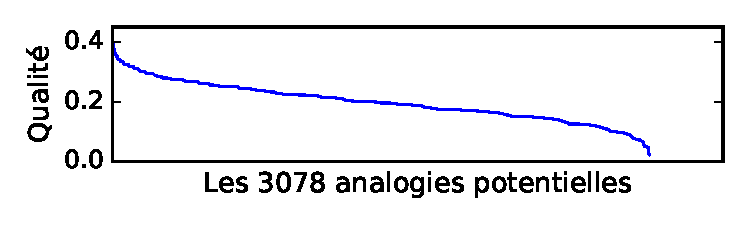
\includegraphics[width=4in]{figures/quality_of_proportions.pdf}
  \caption{Quality of the 993 proportions. The quality of a
  proportion is defined as the fraction of component-proportions that stand
  perfectly.}
\label{FIG:quality_proportions}
\end{figure}
For the best proportions, a perfect analogy stands on more than 70\% of the
components. This is quite significant as we are measuring this fraction over
more than 200 components. However, we have seen that much of these proportions
are not really interesting as all the common users tend to agree on the popular
movies, and the four movies of a proportion tend to be clustered into the same
genre.

To try to exhibit disagreements in the ratings, we used another quality
function. We assign a truth value of $1$ to an analogy $r_1:r_2::r_3:r_4$ if
and only if the proportion complies with one of the following patterns:
\begin{itemize}
  \item $0:1::0:1$,
  \item $1:0::1:0$,
  \item $0:0::1:1$,
  \item $1:1::0:0$.
\end{itemize}
Simply put, we have forbidden the \textit{agreeing analogies} $0:0::0:0$ and
$1:1::1:1$. Figure \ref{FIG:quality_proportions_different_ab_cd} gives us the
fraction of correct proportions for the 993 potential analogies, using this
custom quality function.
\begin{figure}[!h]
\centering
  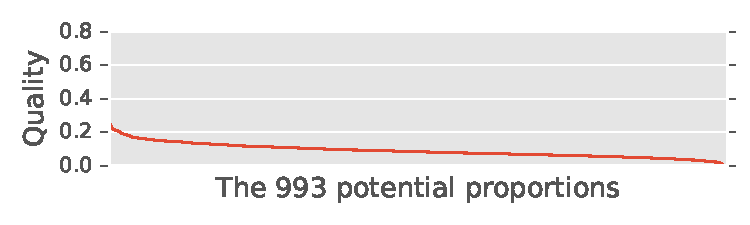
\includegraphics[width=4in]{figures/quality_of_proportions_different.pdf}
  \caption{Quality of the 993 proportions. The quality of a
  proportion is defined as the fraction of components that make up perfect
  proportions, forbidding patterns $0:0::0:0$ and $1:1::1:1$.}
\label{FIG:quality_proportions_different_ab_cd}
\end{figure}
Obviously, the quality drops significantly for the mere reason that we have forbidden patterns
like $r:r::r:r$. This tells us that in fact, \textbf{there are simply not a lot of
interesting analogies}: the best proportion that we found is
\textit{interesting} on less than 25\% of its components, which is quite small.
This confirms our previous observation that sadly, most of the analogies we
find tend to relate four movies that are actual \textbf{neighbors}. We will see
in the conclusion of this chapter how this fact can retrospectively explain the
performances of our basic analogy-based recommender from the first section.

\section*{Conclusion}

In this chapter, we have detailed our contributions to the field of recommender
systems. We have proposed two frameworks based on analogy for the design of
rating prediction algorithms, and also proposed a method for mining analogical
proportions in an incomplete database.

Section \ref{SEC:analogical_reco_basic_algo} described our first attempt at
building an analogy-based prediction algorithm for recommendation. This
algorithm is a direct application of the analogical inference principle, and is
strongly related to the extended classifier that we have described in Chapter
\ref{CHAP:functional_definition}. The basic underlying idea is that if four
users $(a, b, c, d)$ are in analogy regarding their common items (using the
arithmetic proportion), then it should also be the case for other items that
$d$ has not yet rated. We presented a user-based view where analogies were
considered between users, but it is perfectly possible to consider analogies
between items.

We have compared this algorithm with the two main approaches of collaborative
filtering algorithms, namely neighborhood methods and matrix
factorization-based techniques. Our algorithm yields decent accuracy compared
to neighborhood methods, but is extremely expensive in terms of computational
resources.  It was clear that this simple and straightforward application of
the analogical inference principle could not be used in real-world settings,
where computation time is a scarce resource.

These observations led us to consider another framework for analogical
recommendation in Section \ref{SEC:clone_based_view}. Acknowledging the fact
that each user tends to have a very
personal idea of what a good (or bad) rating should be, we introduced the notion of clones
which captures how two users tend to agree semantically on a rating. This
semantic agreement is not necessarily reflected in the numerical rating values:
for a user $u$, the value 3 may
be a good rating, while for $v$ it may be a bad one. We derived two algorithms
relying on this clone-based view of the ratings. We also described a quite
recent technique in collaborative filtering, that allows to address user and
item biases. This method is based on the fact that some users tend to give
higher ratings than others, and some items tend to be rated higher than others.
We discussed how this view (using biases) is related to our view (using
clones), and pointed out the similarities and differences of the two
approaches. It turned out that these two techniques are really close, and the
resemblance is reflected in the algorithms performances. Yet, as the bias-based
method relies on a global optimization problem, it tends to be better at
capturing the overall noise in the data, and still outperforms our method. Our
last contribution to analogical recommendation was to consider an extreme case
of clone-users, considering that the rating scale $[1, 5]$ could be interpreted
as purely ordinal. Unfortunately, this track of research did not lead to
promising results.

In Section \ref{SEC:mining_analogical_proportions}, we proposed an algorithm for the mining of analogical
proportions in a partially described database. This general method perfectly
applies to the problem of mining analogies between users or items in a rating
dataset, such as the one that was used in the first two sections. Based on the
Apriori algorithm, our method is inspired by the mining of association rules
and allows to extract the potential analogies in an efficient way.
We proposed many different quality functions allowing to assess the quality of
a proportion, and naturally some of the quality functions are strongly related
to the Analogical Dissimilarity as defined in Chapter
\ref{CHAP:functional_definition}. We gave
examples of some of the analogies that we found using different variations of
the general mining algorithm, treating ratings as numerical values and as
Boolean values. The main take-away message was that the best analogies that
could be extracted between items were involving users with similar tastes: the four movies of a
proportion were mostly neighbors, in the sense that users tend to agree on
their respective ratings. Also, when forcing proportions to display a
disagreement in the ratings of the four movies, the best proportions that were
revealed still had a pretty bad quality.

This allows us to retrospectively interpret the results of our first
analogy-based prediction algorithm. We have seen that its performances were close to
that of a neighborhood-based technique, but in the light of what has just been
explained we can fairly say that there were no analogies to find in the
database, except for those involving four neighbors. So after all, our
analogy-based inference principle was reduced to that of the classical $k$-NN
approach. Clearly in that case, paying the price of the cubic search in the set
of all users is really not worth it. This is entirely dependent on the database
that was used (in our case, the MovieLens dataset), and we may still presume
that there should exist a dataset where the use of analogical proportion is
beneficial over a simple neighborhood approach.

Even if our investigations on analogical recommendation did not completely live
up to our expectations, there still is a contribution of ours that  is worth
mentioning. As pointed out earlier in the first section, all of our
recommendation experiments
were carried out using Surprise\footnote{\url{http://surpriselib.com}}
\cite{Surprise}, an open source Python recommendation engine that we have
developed. Quite surprisingly, when we started our experiments a few years
ago, there was no Python library that would allow to easily run
cross-validation procedures, or that would make the implementation of a
recommendation algorithm easy. But most importantly, it seemed that most of the
implementation details of the available algorithms were never explicitly
mentioned, so it made comparing performances of the algorithms difficult, if not
meaningless. So we decided to write our own package. We started out by writing
our own custom (and hacky) scripts, which grew up to become a much more
complete and fairly popular recommendation engine. As of April 2017, the main
features of Surprise are the following ones:
\begin{itemize}
  \item Users can have perfect control over their experiments, and to this end
    a strong emphasis was laid on documentation, which we have tried to make as
    clear and precise as possible by pointing out every detail of the
    algorithms.
  \item Dataset handling is made easy. Custom datasets can be used, and the
    MovieLens datasets are natively supported.
  \item Various ready-to-use prediction algorithms are available, such as
    baseline algorithms, neighborhood methods, matrix factorization (SVD,
    PMF, SVD++, NMF), and many others. Also, various similarity measures
    (Cosine, MSD, Pearson \dots) are built-in.
  \item The implementation of new algorithm ideas is made extremely simple.
  \item Cross-validation procedures can be run very easily, as well as
    exhaustive search over a set of parameters for optimization (much like the
    Grid Search feature of the excellent machine learning library scikit-learn
    \cite{scikit-learn}).\\
\end{itemize}

With that, we now close our discussion on analogical recommendation and on
practical applications of analogy. In the next chapter, having these findings
in mind, we will go back to our original theoretical considerations and try to
challenge the analogical inference principle that we have so far ``blindly''
followed.

\paragraph{Résumé du chapitre}

Ce chapitre décrit nos contributions à la recommandation analogique.

Nous avons d'abord décrit nos premières expérimentations relatives  à
l'implémentation d'un algorithme de prédiction de notes fondé sur les
proportions analogiques. Cet algorithme est une application directe du principe
d'inférence analogique, et il est très étroitement lié aux classifieurs étendus
que nous avons décrits dans le chapitre \ref{CHAP:functional_definition}.
L'idée principale derrière cet algorithme est que si quatre utilisateurs $(a,
b, c, d)$ sont en proportion vis-à-vis des items qu'ils ont conjointement notés
(en utilisant la proportion arithmétique), alors cela devrait aussi être le cas
pour d'autres items que $a, b, c$ ont noté mais que $d$ n'a pas encore noté. La
prédiction de la note de $d$ pour ces items est alors le résultat de la
résolution de plusieurs équations analogiques. Notons qu'il est parfaitement
possible de considérer des proportions entre items plutôt que des proportions
entre utilisateurs.

Nous avons comparé cet algorithme avec les deux principales approches de
filtrage collaboratif~: les méthodes par voisinage et les méthodes par
factorisation de matrice. Les performances de notre algorithme sont
raisonnables du point de vue de la précision, comparativement aux méthodes par
voisinage.  Cependant, sa complexité algorithmique leur est bien supérieure et
le rend inadapté à des usages où le temps de calcul est une des contraintes
principales.

Ces observations nous ont conduit à proposer une autre façon d'envisager la
recommandation analogique. Pour cela, nous avons introduit la notion de
\textit{clones} : deux utilisateurs sont des clones s'ils ont tendance à donner
des notes \textit{sémantiquement} équivalentes. Cependant, cette équivalence
sémantique n'est pas forcément reflétée dans les notes : pour un utilisateur
$u$, une note  de $3$ peut représenter une bonne note, alors que pour
l'utilisateur $v$ cela représenterait une mauvaise note, ou juste une note
moyenne. Nous avons proposé deux algorithmes qui suivent cette idée. Nous avons
aussi présenté une contribution récente de technique par filtrage collaboratif
motivée par le fait que certains utilisateurs ont tendance à donner des notes
plus élevées que d'autres, et que certains items ont tendance à être notés avec
plus de clémence. Nous avons expliqué par quels aspects ces deux approches se
rapprochent et diffèrent l'une de l'autre. Du point de vue des performances,
les deux méthodes restent assez similaires avec tout de même un léger avantage
pour les méthodes qui ne reposent pas sur les \textit{clones}.


Enfin, nous avons proposé un algorithme pour la fouille de proportions
analogiques dans des bases de données partiellement complètes. Cette méthode
générale s'applique parfaitement au problème de la fouille de proportions
entre utilisateurs ou entre items, dans une base de notes telle que
celle utilisée dans nos précédentes expérimentations. Notre algorithme est
inspiré de la fouille de règles d'associations et repose sur l'algorithme
Apriori pour extraire des analogies potentielles de manière efficace. Nous
avons proposé diverses fonctions de qualité permettant d'évaluer la qualité d'une
proportion, lesquelles sont très proches de la dissimilarité analogique décrite
dans le chapitre \ref{CHAP:functional_definition}. Nous avons donné divers
exemples de proportions trouvées dans la base de notes, révélant des
proportions entre films. Une des principales observations est que les meilleures
analogies que l'on pouvait extraire de cette base ne mettaient en jeu que des
utilisateurs avec des goûts similaires : les quatre films d'une même
proportion étaient généralement également aimés, ou également rejetés. En ce
sens, on peut considérer que les quatre items d'une même proportion sont en
fait des voisins.

Ceci nous permet d'interpréter rétrospectivement les résultats modestes de nos
premières expérimentations sur la prédiction de note. Nous avons vu que les
résultats de notre algorithme étaient proches de ceux des méthodes par
voisinage, ce qui s'explique maintenant par le fait que les meilleures
proportions dont l'algorithme disposait mettaient en jeu des voisins. En
quelque sorte, notre algorithme analogique était réduit à une approche par
voisinage classique. Il est clair que dans ce cas là, il  n'est pas nécessaire
d'avoir recours à la recommandation analogique, puisque l'on est obligé de
payer le prix d'une complexité cubique. Il reste à noter que ces résultats ont
été obtenus sur la base de données MovieLens : on peut toujours supposer que
sur une autre base, les proportions potentielles restent significatives et
qu'alors l'usage de la recommandation analogique reste intéressant.

Pour finir, permettons-nous de mentionner que nos expérimentations sur la
recommandation nous ont conduit à développer un package Python appelé Surprise
\cite{Surprise} consacré aux algorithmes de prédiction de notes, dont les
principales fonctionnalités sont les suivantes :

\begin{itemize}
  \item Les utilisateurs peuvent avoir un contrôle total sur le protocole
    expérimental mis en oeuvre. A cet effet, une attention particulière a été
    attachée à la documentation, que l'on a essayé de rendre la plus claire
    et détaillée possible.
  \item La gestion des jeux de données est facilitée. Certaines bases de
    données classiques sont pre-intégrées, telle que les bases MovieLens.
  \item Divers algorithmes de prédiction sont implémentés, tels que les
    méthodes de voisinage, des méthodes par factorisation de matrice, et
    d'autres. D'autre part, plusieurs mesures de similarité sont disponibles
    d'office.
  \item La création de nouveaux algorithmes de prédiction est extrêmement simple.
  \item Les procédures de validation croisée sont faciles à implémenter. Une
    autre fonctionnalité intéressante est la possibilité d'effectuer des
    recherches exhaustives sur l'espace des paramètres d'un algorithme, pour
    déterminer la combinaison de paramètres qui produit les meilleurs résultats
    (\textit{grid search}).
\end{itemize}

